\documentclass[11pt, rgb]{scrreprt}
\usepackage{themeKonstanzDBIS} % Muss immer verwendet werden (Standardpaket)

\usepackage{algorithm}
\usepackage{algorithmicx}
\usepackage{algpseudocode}
\usepackage{mathtools}  % amsmath with extensions
\usepackage{amsmath} 
\usepackage{amsfonts}  % (otherwise \mathbb does nothing)
\usepackage{amssymb}  % (otherwise \mathbb does nothing)
\usepackage{nameref}


\format{a4}

% Thesis information        %
%\date{\today}
\year{2023}
\author{Marius Hahn}
\title{MSc Thesis}
\subtitle{thesis}
\unisection{Faculty of Sciences}
\department{Department of Computer and Information Science}
\supervisorOne{Prof. Dr. Theodoros Chondrogiannis}
\supervisorTwo{Prof. Dr. Sabine Storandt}

\headFoot{14}

%%%%%%%%%%%%%%%%%%%%%%%%%%%%%%%%%%%%%%%%%%%%%%%%%%%%%%%%%
% Begin vom Dokument                                    %
%%%%%%%%%%%%%%%%%%%%%%%%%%%%%%%%%%%%%%%%%%%%%%%%%%%%%%%%%

\begin{document}

% Thesis Title
\thesistitlepage[language=english]{MSc Thesis Title}

\chapter*{Abstract}

% Table of Contents           
\tableofcontents

%Use only if thesis is over 100 pages.
% List of figures
%\listoffigures
%\addcontentsline{toc}{chapter}{List of Figures}

%Use only if thesis is over 100 pages.
% List of tables
%\listoftables
%\addcontentsline{toc}{chapter}{List of Tables}

% For chapters and sections use  
%    \chapter{...}
%    \section{...}
%    \subsection{...}
%    \subsubsection{...}
%

\rmfamily 
\normalsize

\chapter{Introduction}

\chapter{Related Work} 

As this is manly a database paper, we want to divide this chapter in two main sections \nameref{sec:algorithmic_history} and \nameref{sec:related_work:database}. \nameref{sec:algorithmic_history} 
will give some basic overview what has been published regarding index structures to speed up shortest path queries for graphs. \nameref{sec:related_work:database} will try 
to give an overview of efforts that have been made to make \cite[Customizable Contraction Hierarchies]{CCH} it suitable for graph databases.

\section[Algorithmic History]{Algorithmic History} \label{sec:algorithmic_history}

\cite[Contraction Hierarchies]{Geisberger_2012} or CH is heavly influenced by the idea of the \cite[Transit-Node]{Bast_2007} approach and as transit node approach itself is a
technique to speed up the \cite[Dijkstra Algorithm]{Dijkstra_1959} which is the most basic and robust algorithm to find shortest path in graphs. CH goes back to the diploma thesis of \cite[Geisberger]{Geisberger} in 2008. The \cite[Transit-Node]{Bast_2007} approach
tries to find vertex inside the graph that are more important than others. Important in this case means, these are vertices that lie on many shortest paths. This speeds up 
especially long distance queries, as one only needs to calculate the distance to the the next transit node of the source and target vertex because the shortest paths between 
the transit or access nodes will be known. \\ 
CH goes even further on the idea of having important vertices. It applies an importance to each vertex in the graph a so called rank. Furthermore it add edges to the graph
, so called shortcut, that preserve the shortest path property of the graph in case a vertex that is contracted lies on a shortest path between other. When querying a shortest
path CH uses a modified bidirectional-dijkstra that is restricted to only visit nodes that are of higher importance, or rank, than the its about to expand next.
This method is able to retrieve shortest paths of vertices that have a high spacial distance, however, it is rather static. In case a new edge is added or an edge weight is updated, 
it might be necessary to recontract the whole graph to preserve the shortest path property. \\
In 2016 \cite[Customization Contraction Hierarchies]{CCH} or CCH was published. The approach is the same, but in CCH shortcuts are not only added if the contraction violtes the shortest,
they are added if there had been a connection between its neighbors through the just contracted vertex and these neighbors do not own a direct connection through an already existing edge.
The shortcut weights are later on calculated through the lowers triangle. Additionally the \cite[Customization Contraction Hierarchies]{CCH} provides an update approach that only updates,
edges that are affected by a weight change.

\section{Contraction Hierarchies Database History}\label{sec:related_work:database}

There is one bachelor thesis by Nicolai D'Effremo \cite[Some text]{DEffremo2019} that has implemented a version on \cite[Contraction Hierarchies]{Geisberger_2012} for Neo4j, one 
of the most used graph databases of today in 2023. This implementation shows that even in CH an index structure is also worth pursuing in a database context, as the speedup 
of shortest path queries paired with a reasonable preprocessing time. \cite{Zickenberg2021} wrote a showed in his bachelor thesis that it is even possible to restricted these
queries with label constraints. Although CH and CCH have little difference, sadly we could not use much of the code provided as it
was deeply integrated into the Neo4j-Platform and since that there have been two major release updates with breaking changes which make it nearly impossible to reuse any of
this code.\\

Finally there is \cite[Mobile Route Planning]{Sanders} by Peter Sanders, Dominik Schultes, and Christian Vetter. In this paper it is described how one can efficiently store
the a CH index structure on a hard drive. It states an interesting technique to how store edge that are likely to be read sequentially spatially close on the hard drive which 
makes read operations that have to be done during query time fast. The motivation of \cite[Mobile Route Planning]{Sanders} through was slightly different. They came up with this
idea because computation power on mobile devices is limited, so they could precalculate the CH index on a server and then later distribute it to a mobile device.

\chapter{Preliminary}

\section{Notation and Expressions}
We denote a graph $G(V, E)$ in case me mean an \textit{undirected} graph, where $v$ is a vertex contained in the vertices $v \epsilon  V$ and $e$ is an edge $e \epsilon E$. An edge is uniquely defined by to vertices $v_a$ and $v_b$ such that $v_a \neq v_b$, so there are no loops nor multi edges. An edge additionally has a weight function $w: E \rightarrow \mathbb{R}_{<0} $ it's weight which must be a positive. 

\section{Customizable Contraction Hierarchies}\label{sec:Preliminary_CCH}

\chapter{Integration in a Neo4j}

In this section it is described how "Customizable Contraction Hierarchies" CCH is integrated into Neo4j. CCH arguments the input graph, which means it inserts arcs, so called shortcuts, that do not belong to the original data. To keep the change to the input graphs as little as possible we decided to not insert any arc into the graph that is stored inside the neo4j database, but introduce another graph data structure, the index graph. This index graph has an mapping to the input graph that is held by the database, by inserting two properties into the node of the input graph. The \textit{rank} this vertex has in the index graph and the \textit{indexing weight} it had during the last customization process. This gives yet another two advantages. One is that we get full control about the graph representation which is helpful to efficiently store and read the index graph for the disk. Another is that the with this approach it makes it easier to later on port the idea to another graph database manufactures.

\section{Index Graph Data Structure}

The index graph data structure is neither a adjacency list nor adjacency matrix. There is a vertex object that has two hash tables. One for incoming arc and one for outgoing arcs. The hash tables keys are of type vertex and the value is the arc. An arc has a reference to its start vertex and one to its end vertex. \\
A disadvantage of this model could be that some modern hardware optimization that exist for arrays do not match with this data structure. When using an array, the values this array are stored sequentially in main memory. When one value of an array is accessed by the CPU, modern hardware reads subsequent values into the CPU-cache because it is likely that they are accessed right after it. The model of the index graph is a linked data structure, a bit like a linked list. The elements of an linked list are contained somewhere in main memory. There is no guarantee that subsequent values have any spacial proximity. Therefore the just explained hardware optimization will not give any advantage. \\ % cite some paper to this topic
However, this makes the makes the graph traversal easy. Additional it makes it very efficient to explore the neighborhood of a vertex. There is no array traversal to find a vertex and only one hash table lookup for finding an arc of a vertex. Additionally these hash tables only contain few elements. This makes this data structure efficient anyway. Test on small graphs [Oldenburg] show that cch queries can be answered in less than one millisecond, which is close to what we tested with the original cch application.

\section{The Contraction}

There are two way to get a suitable vertex order. A so called \textit{metric independent} and a so called \textit{metric dependent} one. The metric independent recursively uses balanced separator to determine a vertex ordering\cite{CCH}. Although this is the superior method, it is not used in this paper writing an algorithm that calculates balanced separators isn't trivial, and we are not aiming for optimizing the contraction process. 

\subsection{Metric Dependent Order}

The metric dependent order mainly uses the edge difference $ED$ to determine which vertex is to be contracted next. The $ED$ is determined as the $|edges To Insert| - |edges To Remove|$. The fewer edges are inserted during contraction the fewer edges will be contained by the final graph. However using only the edge differences doesn't lead to desired result. This is because during contraction there will be areas that get less dense than other. There are two problems that can arise. One is that important vertices are not contracted last. The other is the search space of the query gets linear although it could be logarithmic.

\subsubsection{Important Vertices not contracted last}\label{sec:not_contracted_last}

\begin{figure}
    \centering
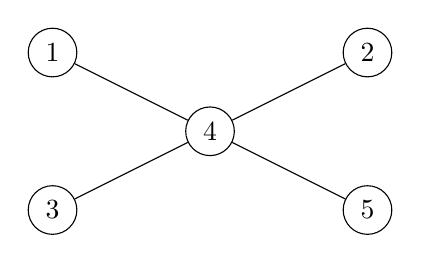
\begin{tikzpicture}[node distance={15mm}, main/.style = {draw, circle}]
\node[main] (x1) at (1, 2) {$1$}; 
\node[main] (x3) at (1, 0) {$3$};

\node[main] (x4) at (3, 1) {$4$}; 

\node[main] (x2) at (5, 2) {$2$}; 
\node[main] (x5) at (5, 0) {$5$}; 

\draw (x1) -- (x4);
\draw (x2) -- (x4);
\draw (x3) -- (x4);
\draw (x5) -- (x4);

\end{tikzpicture} 
    \caption{The numbers inside the vertices represent their contraction order}
    \label{fig:not_contracted_last}
\end{figure}

Looking at figure \ref{fig:not_contracted_last}, this is a possible contraction order, if only the $ED$ is used to contract vertices. At the beginning the nodes with rank 1, 2, 3, 5 have the same edge difference, which is $ED = -1$. One edge will be removed after contraction and the is no shortcut inserted. This happens until there are only the vertices 4 and 5 left. Now vertex 4 has an $ED=-1$, too, same as vertex 5. Therefore the algorithm contracts the vertex with rank 4 before the one with rank 5. \\
However this is not the desired result. There are six ${(1,2), (1,3), (1,5), (2,3), (2,5), (3,5)}$ shortest paths that involve vertex 4, all the other vertices do not encode any shortest path, so vertex 4 should be contracted last. This can be overcome by the method that is explained in section \ref{sec:vertex_importance}

\subsubsection{Linear Query Search Space}\label{sec:linear_query}

\begin{figure}
\centering

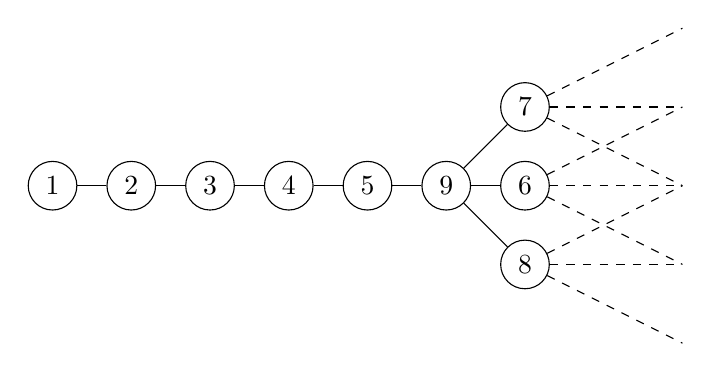
\begin{tikzpicture}[node distance={15mm}, main/.style = {draw, circle}]

\node[main] (x1) at (0, 0) {$1$};
\node[main] (x2) at (1, 0) {$2$};
\node[main] (x3) at (2, 0) {$3$};
\node[main] (x4) at (3, 0) {$4$};
\node[main] (x5) at (4, 0) {$5$};
\node[main] (x9) at (5, 0) {$9$};

\node[main] (x7) at (6, 1) {$7$};
\node[main] (x8) at (6, -1) {$8$};
\node[main] (x6) at (6, 0) {$6$};


\draw (x1) -- (x2);
\draw (x2) -- (x3);
\draw (x3) -- (x4);
\draw (x4) -- (x5);
\draw (x5) -- (x9);

\draw (x6) -- (x9);
\draw (x9) -- (x7);
\draw (x9) -- (x8);

\draw [dashed] (x7) -- (8, 2);
\draw [dashed] (x7) -- (8, 1);
\draw [dashed] (x7) -- (8, 0);

\draw [dashed] (x8) -- (8, 0);
\draw [dashed] (x8) -- (8, -2);
\draw [dashed] (x8) -- (8, -1);

\draw [dashed] (x6) -- (8, 1);
\draw [dashed] (x6) -- (8, 0);
\draw [dashed] (x6) -- (8, -1);

\end{tikzpicture} 
\caption{Linear Contraction}
\label{fig:linear_contraction}
\end{figure}

Looking at figure \ref{fig:linear_contraction} this is a possible contraction order using the only the $ED$ as method to determine the importance of a vertex. As you can see vertex 9 is the one with the highest importance. Which is the desire result as all shortest path come from vertices ${1, 2, 3, 4, 5}$ and go any of the vertices ${6, 7, 8}$ have to pass through vertex 9. However regarding only vertices $1, 2, 3, 4, 5$, there is only one way to go when looking for the shortest path. And if we only go left vertex by vertex, there is no difference between our search or a Dijkstra search. Which means, no gain in query performance. Better would be to contract vertex 3 before vertex 2. This would insert one shortcut more which is bearable in sparse areas, but it decreases the hops that need to be done by one as you insert an arc between vertex 2 and 4, so you can surpass vertex 3. 

\subsection{Vertex importance}\label{sec:vertex_importance}

As shown in section \ref{sec:not_contracted_last} and \ref{sec:linear_query} using only the $ED$ as a metric to determine which vertex to contract next is not sufficient to get a suitable


\section{How to Store the Index Graph}

\begin{figure}
    \centering
    

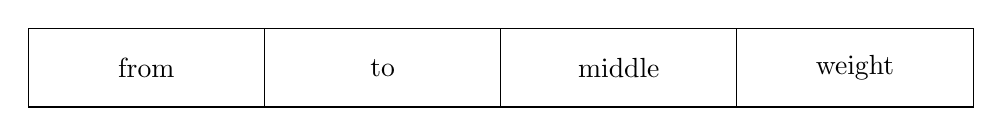
\begin{tikzpicture}[node distance={15mm}, main/.style = {draw, circle}]
    \draw (0,0) rectangle (12,1);
    \draw (3,0) -- (3,1);
    \draw (6,0) -- (6,1);
    \draw (9,0) -- (9,1);
    \node at (1.5, 0.5) {from};
    \node at (4.5, 0.5) {to};
    \node at (7.5, 0.5) {middle};
    \node at (10.5, 0.5) {weight};

\end{tikzpicture}
    \caption{Single Record}
    \label{fig:singleRecord}
\end{figure}

\begin{figure}
    \centering
    
    \begin{tikzpicture}[node distance={15mm}, main/.style = {draw, circle}]
        \draw (0,7) -- (4,7);
        \draw[dashed] (0,6) -- (4,6);
        \draw[dashed] (0,5) -- (4,5);
        \node at (4.5,5) {0};
        \node at (4.5,1) {1};
        \draw (0,3) -- (5,3); 
        \draw[dashed] (0,2) -- (4,2);
        \draw[dashed] (0,1) -- (4,1);
        \draw[out=60, in=-120] (0,0) to (4, 0);
        \draw (0,0) -- (0,7); 
        \draw (4,0) -- (4,7); 
        \node at (2, 6.5) {record};
        \node at (2, 5.5) {record};
        \node[rotate=90, font=\Large] at (2, 4) {. . . . .};
        \node[rotate=90] at (-0.85, 5) {disk block};
        \draw [decorate,decoration = {brace, amplitude=10pt}] (-0.2,3) --  (-0.2,7);
    \end{tikzpicture}
    
    \caption{Disk Block}
    \label{fig:disk_block}
\end{figure}


\chapter{Important Algorithms}

\subsection{Updating a Priority Queue}

\section{Search Algorithm}


\newpage
\section{Triangles}

\begin{figure}
    \centering

\begin{tikzpicture}[node distance={15mm}, main/.style = {draw, circle}]
\node[rotate=90] at (-0.25,0) {rank};
\draw [ -Stealth]  (0,-2) -- (0,2);
\node[main] (x1) at (1, 0) {$x$}; 
\node[main] (z1) [below right of=x1] {$z$};
\node[main] (y1) [right of=z1, above of=x1] {$y$}; 
\draw (x1) -- node[above left, sloped] {$a$} (y1) ;
\draw (x1) -- node[below left, sloped, pos=0.8] {$b$} (z1);
\draw (y1) -- node[below left, sloped] {$c$} (z1);
\node[] at (2,-2) {lower triangle $\{x,y\}$};

\node[main] (z2) at (6, 0) {$z$}; 
\node[main] (x2) [below right of=z2] {$x$};
\node[main] (y2) [right of=z2, above of=z2] {$y$}; 
\draw (z2) -- node[above left, sloped] {$c$} (y2) ;
\draw (z2) -- node[below left, sloped, pos=0.8] {$b$} (x2);
\draw (y2) -- node[below left, sloped] {$a$} (x2);
\node[] at (7,-2) {intermediate triangle $\{x,y\}$};

\node[main] (y3) at (12, 0) {$y$}; 
\node[main] (x3) [below right of=y3] {$x$};
\node[main] (z3) [right of=y3, above of=y3] {$z$}; 
\draw (y3) -- node[above left, sloped] {$c$} (z3);
\draw (y3) -- node[below left, sloped, pos=0.8] {$b$} (x3);
\draw (z3) -- node[below left, sloped] {$a$} (x3);
\node[] at (13,-2) {upper Triangle $\{x,y\}$};
\end{tikzpicture}

    \caption{Triangle Enumeration}
    \label{fig:triangel enumeration}
\end{figure}

\begin{algorithm}
\caption{Compute Triangles}
\begin{algorithmic}[1]

\Procedure{lowerTriangles}{$arc, neighbors$}
\State $\text{triangles} \gets$ \{\}; 
$\text{x} \gets$ min(arc.start, arc.end);
$\text{y} \gets$ max(arc.start, arc.end);
\ForAll{$z$ in $neighbors$}
    \If{$z < x < y$}
        \If{$\text{upwards}(arc)$}
             $\text{triangles.add}(\text{Triangle}(arc, x.\text{getArcTo}(z), z.\text{getArcTo}(y)))$
        \Else  $\text{ triangles.add}(\text{Triangle}(arc, z.\text{getArcTo}(x), y.\text{getArcTo}(z)))$
        \EndIf
    \EndIf
\EndFor
\State \textbf{return} $\text{triangles}$
\EndProcedure

\Procedure{intermediateTriangles}{$arc, neighbors$}
\State $\text{triangles} \gets$ \{\};
$\text{x} \gets$ min(arc.start, arc.end);
$\text{y} \gets$ max(arc.start, arc.end);
\ForAll{$z$ in $neighbors$}
    \If{$x < z < y$}
        \If{$\text{upwards}(arc)$}
             $\text{triangles.add}(\text{Triangle}(arc, z.\text{getArcTo}(x), z.\text{getArcTo}(y)))$
        \Else  $\text{ triangles.add}(\text{Triangle}(arc, x.\text{getArcTo}(z), y.\text{getArcTo}(z)))$
        \EndIf
    \EndIf
\EndFor
\State \textbf{return} $\text{triangles}$
\EndProcedure

\Procedure{upperTriangles}{$arc, neighbors$}
\State $\text{triangles} \gets$ \{\};
$\text{x} \gets$ min(arc.start, arc.end);
$\text{y} \gets$ max(arc.start, arc.end);
\ForAll{$z$ in $neighbors$}
    \If{$x < y < z$}
        \If{$\text{upwards}(arc)$}
             $\text{triangles.add}(\text{Triangle}(arc, z.\text{getArcTo}(x), z.\text{getArcTo}(y)))$
        \Else  $\text{ triangles.add}(\text{Triangle}(arc, x.\text{getArcTo}(z), y.\text{getArcTo}(z)))$
        \EndIf
    \EndIf
\EndFor
\State \textbf{return} $\text{triangles}$
\EndProcedure

\end{algorithmic}
\end{algorithm}




\bibliography{related.bib}
\addcontentsline{toc}{chapter}{Bibliography}


\end{document}
